\documentclass[11pt,addpoints,answers]{exam}
%\noprintanswers % Change to \printanswers to show solutions
\usepackage{soul}
\usepackage{amsmath}
\usepackage{graphicx}
\usepackage{tikz}
\usepackage{pgfplots}
\usetikzlibrary{positioning}

\title{Mid-Term Exam}
\author{Sadamori Kojaku}
\date{\today}
\newenvironment{explanation}{\expandafter\comment}{\expandafter\endcomment}
\usepackage{verbatim}

\begin{document}

\pagestyle{head}
\firstpageheader{Applied Soft Computing}{Mid-Term Exam}{\today}
\runningheader{Applied Soft Computing}{Mid-Term Exam}{Page \thepage\ of \numpages}

\begin{center}
  \fbox{\fbox{\parbox{5.5in}{
    \textbf{Instructions:} Answer all questions. Show all work.
    Total: \numpoints\ points.
  }}}
\end{center}

\vspace{0.2in}

\makebox[0.5\textwidth]{Name:\enspace\hrulefill}

\begin{questions}

\question[1] One represents words as vectors of zeros with a single one at the position corresponding to the word.
This is known as \fillin[one-hot encoding].
\begin{solution}
One-hot encoding.
\end{solution}

\question[1] ``You shall know a word by the company it keeps'' is a famous quote that explains the idea that word meaning can be derived from the context in which a word appears. This idea is known as the \fillin[distributional] hypothesis.
\begin{solution}
The distributional hypothesis is a key principle suggesting that words appearing in similar contexts have similar meanings. By analyzing the surrounding words, the model can understand the relationship between words. This is a critical distinction because the distributional hypothesis forms the basis for techniques like TF-IDF and word embeddings, which aim to encode semantic relationships.
\end{solution}

%\question[2] In the context of Word2Vec, the \fillin[CBOW] model predicts the center word based on its surrounding context words, while the \fillin[Skip-gram] model predicts the surrounding context words given a center word.
%\begin{solution}
%  \begin{itemize}
%    \item CBOW (Continuous Bag of Words): This model takes the surrounding context words as input and tries to predict the center word. The example in the text "The \_\_\_\_\_ chases mice in the garden" illustrates this. It's a fill-in-the-blank task where you're predicting the missing word.
%    \item Skip-gram: This model does the reverse. Given a center word, it tries to predict the surrounding context words. The example in the text is "\_\_\_\_\_ cat \_\_\_\_\_ \_\_\_\_\_ \_\_\_\_\_ \_\_\_\_\_ ".
%  \end{itemize}
%  The question is clearly worded and tests understanding of the core difference between the two models. It directly addresses their prediction tasks, as described in the document.
%\end{solution}

%\question[1] In the SemAxis framework, a semantic axis is defined by a pair of \fillin[antonymous] words in the word embedding space.
%\begin{solution}
%The correct answer is "antonymous." The SemAxis framework explicitly defines semantic axes using pairs of antonymous (opposite-meaning) words, as stated in the core concept definition in the document. Other options are not relevant to the core definition of how axes are defined.
%\end{solution}

\question[1] In the context of training RNNs, the process of computing gradients back through time is known as \fillin[Backpropagation Through Time (BPTT)].
\begin{solution}
BPTT is the method used to compute gradients in RNNs, unfolding the network through time and applying backpropagation.
\end{solution}

\question[1] In the context of training RNNs, the gradients become extremely small as they are backpropagated through many time steps. This is known as the \fillin[vanishing gradient] problem.
\begin{solution}
The vanishing gradient problem occurs when the gradients become extremely small as they are backpropagated through many time steps, making it difficult for the network to update its weights effectively and learn long-term dependencies.
\end{solution}

\question[3] The three main gates in an LSTM cell are the forget gate, the input gate, and the output gate. The \fillin[forget] gate decides what information to remove from the cell state, the \fillin[input] gate determines what new information to store in the cell state, and the \fillin[output] gate controls what parts of the cell state should be revealed as output.
\begin{solution}
The forget gate examines the current input and the previous hidden state to decide what information to remove from the cell state. The input gate works together with a candidate memory generator to decide what new information to store. The output gate controls what parts of the cell state should be revealed as output. These three gates work together to control the flow of information within the LSTM cell, allowing it to maintain long-term dependencies.
\end{solution}

\question[1] \fillin[Dropout] is a technique used to mitigate overfitting by randomly deactivating a portion of the neurons during the training process.
\begin{solution}
Dropout is a regularization technique used in neural networks, including LSTMs, to prevent overfitting. It randomly deactivates (sets to zero) a fraction of neurons during training. This forces the network to learn more robust features and reduces its reliance on specific neurons. This concept is discussed in the content, and the visual aid clarifies the impact of the regularization.
\end{solution}

\question[1] In the ELMo architecture, the \fillin[bidirectional] LSTM processes text in both forward and backward directions to generate word representations.
\begin{solution}
Bidirectional LSTM processes text in both forward and backward directions. The forward LSTM processes the words from the first to the last, while the backward LSTM processes the words from the last to the first. The two LSTM outputs are then concatenated to form a single vector representation for each word.
\end{solution}

\question[1] In the attention mechanism, the context vector is computed as a \fillin[weighted sum] of the encoder hidden states using the attention weights.
\begin{solution}
The context vector is calculated as a weighted sum of the encoder hidden states using the attention weights. This is the core functionality of the attention mechanism, allowing the model to focus on the relevant parts of the input sequence. The attention weights determine how much each hidden state contributes to the context vector, effectively enabling the model to 'pay attention' to the most important parts of the input when generating the output. Other options are not appropriate since they don't represent the method the context vector is computed.
\end{solution}

\question[2] In the decoder transformer block, the \fillin[masked attention] mechanism prevents the model from accessing future tokens during training, while the \fillin[cross-attention] mechanism allows the decoder to attend to the encoder's output for tasks like translation.
\begin{solution}
  \begin{itemize}
    \item Masked Multi-Head Attention: This mechanism is essential for the parallel training of the decoder. By masking future tokens during training, it ensures the model learns to generate output sequentially, preventing it from "peeking" at the future, and it can also act as regular attention mechanism during the inference. This is critical for ensuring the model learns to generate tokens in the correct order, which can be more efficient and prevent error accumulation problems.
    \item Cross-Attention: Cross-attention allows the decoder to access information from the encoder's output. It enables the decoder to focus on the relevant parts of the input sequence, which is essential for tasks like translation, where the decoder needs to understand the meaning of the input to generate the correct output. For instance, in translating "I love you" to "Je t'aime", cross-attention allows each French word to focus on related English words (e.g., "Je" attending to "I" and "t'aime" to "love").
  \end{itemize}
\end{solution}

\question[3] In the self-attention mechanism, the attention score is computed using the \fillin[query] vectors and \fillin[key] vectors, and then normalized using the softmax function. This score is then used to calculate a weighted sum of the \fillin[value] vectors to produce the contextualized vector.
\begin{solution}
  \begin{itemize}
    \item Query, Key, and Value Vectors: These are the fundamental components of the self-attention mechanism. Each word in a sequence is transformed into these three vectors. The query vector is used to represent the word when it is searching for relevant information, the key vector is used to represent the word when it is being searched for, and the value vector contains the information to be retrieved. The attention score measures the relationship between query and key vectors. The value vectors are then weighted by the attention scores to produce the contextualized vector. The query and key vectors are used to compute the attention score by taking a dot product of them. The attention scores are then normalized using the softmax function to provide the weights. The weighted sum of the value vectors is then computed using these softmax weights, which leads to the contextualized vector.
    \item Contextualization: The purpose of the attention mechanism is to contextualize the word vectors, so that each word vector contains the context of the surrounding words. The concept is explained in the document by saying "The output of the attention mechanism is the *contextualized vector*, meaning that the vector for a word can vary depending on other words input to the attention module."
  \end{itemize}
\end{solution}


%\question[1] In the context of generating structured output with LLMs, such as JSON, the technique of specifying a JSON schema and instructing the model to adhere to it during token generation is known as \fillin[constrained sampling].
%\begin{solution}
%Constrained sampling is a method for ensuring that the model's generated text complies with the schema, producing JSON that conforms to a valid structure.
%\end{solution}

%\question[1] In the context of TF-IDF, what is the primary role of the Inverse Document Frequency (IDF) component?
%  \begin{choices}
%    \choice To normalize the frequency of a word within a specific document.
%    \choice To give more weight to words that appear frequently across all documents.
%    \choice To downweight words that appear in many documents, highlighting those unique to a few.
%    \choice To calculate the total number of times a word appears in a collection of documents.
%\end{choices}
%\begin{solution}
%C. IDF's main goal is to reduce the impact of common words (like "the," "a," "is") that appear frequently across all documents. By doing so, it emphasizes the importance of words that are specific to certain documents, which are more likely to be relevant to the topic of those documents. This weighting is mathematically achieved by taking the logarithm of the inverse of the document frequency (number of documents containing the word).
%
%Incorrect options:
%\begin{itemize}
%  \item (A) "To normalize the frequency of a word within a specific document." This describes the function of Term Frequency (TF), not IDF. TF normalizes for document length.
%  \item (B) "To give more weight to words that appear frequently across all documents." This is the opposite of what IDF does. IDF reduces the weight of common words.
%  \item (D) "To calculate the total number of times a word appears in a collection of documents." This is the function of simple word counts across documents, but it is not the function of IDF. TF-IDF uses term frequencies, but IDF itself is a separate calculation.
%\end{itemize}
%\end{solution}

\question[1] Which of the following is a primary limitation of TF-IDF as a word embedding technique, as discussed in the context?
  \begin{choices}
    \choice It fails to account for the frequency of words within a document.
    \choice It does not capture the relationships between words that appear within the same document.
    \choice It is computationally too expensive for large datasets.
    \choice It overemphasizes the importance of common words like 'the' and 'a'.
  \end{choices}
\begin{solution}
B. TF-IDF focuses on the importance of a word to a document, not on the relationships between words in that document. This is explicitly mentioned in the text when discussing TF-IDF's limitations.

The other options are incorrect because:
\begin{itemize}
  \item (A) TF-IDF *does* account for word frequency within a document through the Term Frequency (TF) component.
  \item (C) TF-IDF is not computationally too expensive; it's a relatively efficient technique.
  \item (D) TF-IDF *addresses* the overemphasis on common words through the Inverse Document Frequency (IDF) component, which downweights them.
\end{itemize}
\end{solution}

\question[1] In the context of Word2Vec, the Skip-gram model focuses on local context windows. Which of the following best describes its primary function and how it relates to the overall goal of word embedding?
  \begin{choices}
    \choice Skip-gram predicts the center word given the surrounding context words, and it aims to create a sparse matrix of word-document counts for each word.
    \choice Skip-gram predicts the surrounding context words given a center word, and it aims to learn dense vector representations of words by factorizing a pointwise mutual information matrix.
    \choice Skip-gram predicts the center word given the surrounding context words, and it is primarily used to categorize the input words, and create a sparse matrix of word-document counts for each word.
    \choice Skip-gram predicts the surrounding context words given a center word, and it primarily aims to create a vocabulary of words used in the text.
  \end{choices}
\begin{solution}
  B. Skip-gram predicts the surrounding context words given a center word, and it aims to learn dense vector representations of words by factorizing a pointwise mutual information matrix.

  The core functionality of the Skip-gram model is predicting context words given a center word. It correctly links the model's objective to learning dense vector representations, which is achieved through the factorization of the pointwise mutual information matrix. The other options are incorrect because they either misrepresent the model's prediction task (predicting the center word instead of the context words) or misconstrue its goals (creating a sparse matrix or just a vocabulary). The core idea is to use local context to generate word embeddings.
\end{solution}

\question[1] In the context of Word2Vec, which statement best describes the primary difference between the CBOW (Continuous Bag of Words) and Skip-gram models?
  \begin{choices}
    \choice CBOW predicts the context words given a center word, while Skip-gram predicts the center word given the context words.
    \choice Both CBOW and Skip-gram predict the center word given the context words, but they use different algorithms.
    \choice CBOW predicts the center word given the context words, while Skip-gram predicts the context words given a center word.
    \choice Skip-gram uses a bag-of-words approach, whereas CBOW considers the order of words in the context.
  \end{choices}
\begin{solution}
C.  CBOW (Continuous Bag of Words) is designed to predict a target word (the center word) based on its surrounding context words. Skip-gram, conversely, attempts to predict the surrounding context words given a specific target word (the center word). The other options are incorrect. Option 1 reverses the roles of CBOW and Skip-gram. Option 2 is wrong because the prediction tasks are different. Option 4 confuses the general approach with the specifics of each model; both models, in their basic implementations, do not account for word order directly.
\end{solution}

%\question[1] In the Word2Vec architecture, what is the primary function of the hidden layer?
%  \begin{choices}
%    \choice To directly represent the input word in a one-hot encoded vector.
%    \choice To calculate the probability of each word in the vocabulary appearing in the context.
%    \choice To transform the input word into a dense vector representation, capturing semantic meaning.
%    \choice To act as a lookup table for the co-occurrence matrix of words in the entire corpus.
%  \end{choices}
%\begin{solution}
%C. The correct answer is: "To transform the input word into a dense vector representation, capturing semantic meaning." The hidden layer is the core of the word embedding process. It maps the input word (represented as a one-hot vector) to a lower-dimensional space, creating a dense vector that represents the word's semantic meaning. This dense vector is also known as the word embedding. The other options are incorrect. The input layer is the one-hot vector representation. The output layer is used for predicting context words (in Skip-gram) or the center word (in CBOW). The co-occurrence matrix is not directly represented in the hidden layer, but rather, the hidden layer learns the information that could be derived from the matrix.
%\end{solution}

%\question[1] A researcher is studying the semantic shift of the word ``fast'' in the context of technology news versus sports news. They want to use SemAxis to analyze this. Which of the following is the MOST appropriate first step?
%  \begin{choices}
%    \choice Look at the nearest words of ``fast'' in the embedding space.
%    \choice Define a semantic axis using the words ``fast'' and ``slow''.
%    \choice Calculate the cosine similarity of ``fast'' with other words in the embedding space.
%    \choice Use a domain expert to label the words in the embedding space.
%  \end{choices}
%\begin{solution}
%B. The core of SemAxis is built around defining axes. A semantic axis is created by using a pair of antonymous words (pole words). In this context, the researcher wants to study how 'fast' shifts in meaning. Thus, the best approach is to define an axis using 'fast' and its antonym, 'slow'.
%
%  The other options are incorrect for the following reasons:
%
%  \begin{itemize}
%    \item 'Download a pre-trained word embedding model.' While necessary, this is a prerequisite step. The question asks for the *first* step in *analyzing* with SemAxis. The question assumes that the embeddings are already available (as stated in the hands-on exercise), the next step is using the axes.
%    \item 'Calculate the cosine similarity of 'fast' with other words in the embedding space.' This is how the semantic alignment is *measured* *after* the axis is defined. It's not the first step in creating an axis.
%    \item 'Use a domain expert to label the words in the embedding space.' The domain expert could be helpful later on, to validate the axes. They are not needed to perform the first step.
%  \end{itemize}
%  This question requires critical thinking because it asks the student to apply the concept of semantic axes to a practical scenario. This also addresses the application of semantic axes in different domains, as highlighted in the motivation and background of the original text.
%\end{solution}

%\question[1] In the context of SemAxis, you want to create a ``happy-sad'' semantic axis. You've identified ``happy'' and ``sad'' as initial pole words. You want a robust axis. Which of the following approaches is MOST LIKELY to result in a more reliable and representative axis?
%  \begin{choices}
%    \choice Directly use the vector difference between the words ``happy'' and ``sad''.
%    \choice Compute the cosine similarity of all words in the embedding space to ``happy'' and ``sad'' and create an axis using the words with the highest similarity scores.
%    \choice Find the synonyms of ``happy'' and ``sad'', compute the centroid vector of each set of synonyms, and then define the axis as the difference between the centroid vectors.
%    \choice Manually select 10 antonym pairs and create a semantic axis for each, and average the vectors.
%  \end{choices}
%\begin{solution}
%C. The correct answer is to find the synonyms of ``happy'' and ``sad'', compute the centroid vector of each set of synonyms, and then define the axis as the difference between the centroid vectors. This reflects the robust axis creation method described in the content. This method uses the words that share similar meaning as the polar words to form a concept-based axis.
%\end{solution}

\question[1] In the forward pass of a standard RNN, what is the correct sequence of operations applied to the input data ($x_t$) and the previous hidden state ($h_{t-1}$) to produce the output ($o_t$) at a given time step?
  \begin{choices}
    \choice Concatenation of $x_t$ and $h_{t-1}$, followed by a linear transformation to get the hidden state ($h_t$), then a tanh transformation of $h_t$ to get $o_t$.
    \choice Linear transformation of $x_t$ and $h_{t-1}$ separately, followed by a tanh transformation of the concatenation to get the hidden state ($h_t$), and finally, a linear transformation of $h_t$ to get $o_t$.
    \choice A linear transformation of $x_t$ followed by a linear transformation of $h_{t-1}$, and then summing the results to generate $o_t$ and $h_t$.
    \choice The input ($x_t$) is directly transformed to produce $o_t$, and $h_{t-1}$ is ignored.
  \end{choices}
\begin{solution}
A. As described in the content, the forward pass of an RNN involves concatenating the current input ($x_t$) and the previous hidden state ($h_{t-1}$) into a combined vector ($v_t$). This vector then undergoes a linear transformation (using weight matrix $W_h$ and bias $b_h$) and is passed through the tanh activation function to produce the new hidden state ($h_t$). Finally, $h_t$ is transformed using the output weight matrix $W_o$ to generate the output ($o_t$). The other options are incorrect because they misrepresent the order or the specific transformations involved. The key steps, as shown in the Model section, are concatenation, transformation to $h_t$ using tanh, and then output transformation.
\end{solution}

%\question[1] In an LSTM cell, what is the primary function of the output gate?
%  \begin{choices}
%    \choice To determine what new information should be added to the cell state.
%    \choice To decide which information to remove from the cell state.
%    \choice To control how much of the cell state is revealed as output.
%    \choice To combine the input and previous hidden state to generate a candidate memory.
%  \end{choices}
%\begin{solution}
%  C.
%  \begin{itemize}
%    \item "To determine what new information should be added to the cell state." - This is the function of the input gate and the candidate memory generator. The input gate determines which parts of the candidate memory will be added, and the candidate memory generates the new information.
%    \item "To decide which information to remove from the cell state." - This is the function of the forget gate. The forget gate decides which parts of the cell state to forget based on the current input and previous hidden state.
%    \item "To combine the input and previous hidden state to generate a candidate memory." - This is the function of the candidate memory, which uses the input and hidden state to generate new information that the input gate may choose to add.
%  \end{itemize}
%\end{solution}
%
%\question[1] Which of the following best describes the primary function of the forget gate in an LSTM network?
%  \begin{choices}
%    \choice To determine how much of the previous cell state to discard or retain, based on the current input and previous hidden state.
%    \choice To decide which new information, proposed by the candidate memory, should be added to the cell state.
%    \choice To determine how much of the previous cell state to discard or retain, based on the current input only.
%    \choice To generate new candidate memory values that could be added to the cell state.
%  \end{choices}
%\begin{solution}
%A.
%The forget gate's fundamental role is to selectively erase or preserve information from the cell state based on inputs. This is explicitly described in the text: 'The *forget gate* examines the current input and the previous hidden state to decide what information to remove from the cell state.' The other options describe the functions of the input gate, output gate, and candidate memory, respectively. For example, the input gate decides what new information should be added, and the output gate controls the hidden state output.
%\end{solution}

\question[1] In a sequence-to-sequence model with the attention mechanism, what is the primary function of the context vector when decoding?
  \begin{choices}
    \choice To store the entire input sequence without any compression.
    \choice To directly predict the output sequence without any further processing by the decoder.
    \choice To initialize the decoder's hidden state and provide a weighted summary of the input sequence.
    \choice To act as a fixed-size bottleneck preventing the decoder from accessing relevant information.
  \end{choices}
\begin{solution}
C. The context vector, in the presence of attention, provides a weighted sum of the encoder's hidden states to the decoder, which allows the decoder to focus on different parts of the input sequence when generating the output. This initialization helps the decoder understand the overall meaning of the input and generate an appropriate output sequence. The other options are incorrect because:
  \begin{itemize}
    \item The context vector does not store the entire sequence without compression.
    \item The context vector doesn't directly predict the output sequence. The decoder processes the context vector.
    \item In an attention-based model, the context vector doesn't act as a bottleneck, which is a limitation of the basic seq2seq without attention.
  \end{itemize}
\end{solution}

\question[1] In the BERT architecture, what is the primary function of the [CLS] token?
  \begin{choices}
    \choice To mark the end of a sentence.
    \choice To represent masked words during the Masked Language Modeling pre-training.
    \choice To classify the input sentence as a whole.
    \choice To separate sentences in a pair.
  \end{choices}
\begin{solution}
  C. The correct answer is 'To classify the input sentence as a whole.' As detailed in the 'Special tokens' section, the [CLS] token's final hidden state is used for sentence-level classification tasks.
  \begin{itemize}
    \item 'To mark the end of a sentence' is incorrect. The [SEP] token marks the end of a sentence.
    \item 'To represent masked words during the Masked Language Modeling (MLM) pre-training' is also incorrect. The [MASK] token is used during MLM.
    \item 'To separate sentences in a pair, similar to the [SEP] token' is incorrect. While [SEP] separates sentences, [CLS] is for overall sentence representation.
  \end{itemize}
\end{solution}

\question[1] Sentence-BERT is primarily designed to improve performance in which of the following NLP tasks, compared to a standard BERT model?
  \begin{choices}
    \choice Generating human-quality text.
    \choice Classifying individual words in a sentence.
    \choice Performing tasks that require sentence-level understanding, such as semantic similarity.
    \choice Training the BERT model from scratch.
  \end{choices}
\begin{solution}
C. The correct answer is 'Performing tasks that require sentence-level understanding, such as semantic similarity.' Sentence-BERT is specifically designed for tasks that benefit from understanding the meaning of sentences, such as determining semantic similarity, paraphrase identification, and information retrieval. It modifies BERT to produce sentence embeddings that are semantically meaningful, making it ideal for tasks requiring sentence-level context.

  Incorrect options:
  \begin{itemize}
    \item 'Generating human-quality text' is more closely associated with language generation models, such as GPT. While BERT can contribute to these tasks, it is not its primary focus.
    \item 'Classifying individual words in a sentence' is a task typically performed by models designed for word-level understanding, such as token classification tasks, not the primary strength of Sentence-BERT.
    \item 'Training the BERT model from scratch' is the initial step of BERT models, but it's not a task that Sentence-BERT focuses on. Sentence-BERT builds upon pre-trained BERT models, finetuning them for sentence-level tasks.
  \end{itemize}
\end{solution}

\question[1] Which of the following best describes the key architectural difference between Generative Pre-trained Transformer (GPT) and Bidirectional Encoder Representations from Transformers (BERT) in the context of language modeling?
  \begin{choices}
    \choice GPT uses a bidirectional attention mechanism like BERT, allowing it to consider the entire input sequence simultaneously.
    \choice BERT uses a decoder-only transformer architecture, while GPT utilizes an encoder-decoder architecture.
    \choice GPT employs a causal (unidirectional) attention mechanism, enabling it to generate text autoregressively, while BERT uses bidirectional attention.
    \choice Both GPT and BERT use the same transformer architecture, with differences only in the pre-training objectives.
  \end{choices}
\begin{solution}C
C.
  Incorrect options are incorrect because:
  \begin{itemize}
    \item Option 1: GPT does not use bidirectional attention; it uses causal attention.
    \item Option 2: BERT uses an encoder, not a decoder-only architecture. GPT uses a decoder-only architecture.
    \item Option 4: While pre-training objectives differ, the architectural difference is fundamental; causal vs. bidirectional attention.
  \end{itemize}
\end{solution}

\question[1] Considering the autoregressive nature of GPT and its next-token prediction objective, which of the following statements best describes the primary advantage of nucleus sampling over greedy search in text generation?
  \begin{choices}
    \choice Nucleus sampling guarantees more grammatically correct sentences compared to greedy search.
    \choice Nucleus sampling ensures that the generated text always adheres to the context window length, unlike greedy search.
    \choice Nucleus sampling promotes greater diversity and reduces the likelihood of repetitive text compared to greedy search.
    \choice Nucleus sampling is computationally faster than greedy search, enabling quicker text generation.
  \end{choices}
\begin{solution}
C.
The core advantage of nucleus sampling, as highlighted in the text, is its ability to balance text quality and diversity. Greedy search, by always picking the most probable token, often leads to repetitive or predictable outputs. Nucleus sampling, by sampling from a dynamic set of tokens based on cumulative probability, introduces randomness and allows the model to explore a broader range of possibilities, thereby generating more varied and less repetitive text. The other options are incorrect because: Nucleus sampling does not guarantee grammatical correctness, ensure the length, or faster speed.
\end{solution}

\question[1] Which of the following best describes the MAIN advantage of FLAN-T5 over T5 in the context of instruction-following?
  \begin{choices}
    \choice FLAN-T5 uses a larger dataset for training, leading to improved performance.
    \choice FLAN-T5 is based on a different model architecture compared to T5, enabling it to better interpret instructions.
    \choice FLAN-T5 is explicitly fine-tuned to understand and follow diverse, detailed natural language instructions, unlike T5.
    \choice FLAN-T5 incorporates Reinforcement Learning with Human Feedback (RLHF), allowing for more nuanced responses.
  \end{choices}
\begin{solution}
C.
  \begin{itemize}
    \item The dataset size is not the main difference; both models are based on the T5 architecture.
    \item RLHF is a further development, but not the defining characteristic that separates FLAN-T5 from T5.
  \end{itemize}
  This question avoids common misconceptions by directly addressing the key differences in instruction handling between T5 and FLAN-T5, which is core to the content.
\end{solution}

%\question[1] A user is creating a prompt to extract the names of all the people mentioned in a paragraph. Which component of instruction-based prompting is MOST crucial to ensure the LLM provides the names in a consistent and predictable format, such as a comma-separated list, rather than free-form text?
%\begin{choices}
%  \choice Instruction
%  \choice Data
%  \choice Output Indicator
%  \choice Persona
%\end{choices}
%\begin{solution}
%C. The output indicator is the component specifically designed to specify the desired output format. It tells the LLM how to structure the answer. Without it, the LLM might provide the names in a different order each time or in a descriptive paragraph, which would be inconsistent and not as useful. The Instruction, Data, and Persona are all useful parts of a prompt, but they don't directly control the format of the output. The Instruction gives the task. The Data gives the text to analyze, and the Persona changes the tone of the response.
%\end{solution}

%\question[1] When employing personas in prompts for Large Language Models (LLMs), what is the primary benefit, and what potential risks should be considered?
%
%\begin{choices}
%  \choice The primary benefit is to enhance the factual accuracy of the LLM's responses, while the risk is the potential for increased computational complexity.
%  \choice The primary benefit is to ensure consistent output formatting, and the risk is that the LLM may generate responses in an arbitrary format.
%  \choice The primary benefit is to modulate the tone and style of the LLM's output, such as formality or friendliness, while the risk involves the reinforcement of societal stereotypes or biases.
%  \choice The primary benefit is to improve the LLM's ability to understand complex instructions, and the risk is a higher likelihood of the LLM generating incorrect information.
%\end{choices}
%\begin{solution}
%C. Using personas primarily influences the tone and style (formality, friendliness) of the LLM's output. The risk is the potential for reinforcing societal stereotypes. The content explicitly mentions that adding a persona is helpful when we want to change the tone and style of the response.  It also touches upon the bias in LLMs, stating that when prompted to adopt specific socio-demographic personas, LLMs may produce responses that reflect societal stereotypes.  The other options are incorrect because: A is incorrect, the goal of a persona is to change the tone and style, and it will not affect the computational complexity. B is wrong because persona will change the tone and style not the output formatting. D is incorrect, personas are designed to modulate the style or tone and not directly help with understanding complex instructions, or the generation of factual errors.
%\end{solution}

%\question[1] Which of the following scenarios BEST illustrates how chain prompting enhances an LLM's ability to generate a detailed and specific smartphone review?
%
%\begin{choices}
%  \choice The LLM generates a full review in a single prompt.
%  \choice The LLM produces the review step-by-step by sequentially such as analyzing design, performance, camera, and battery life, integrating each assessment into the final review.
%  \choice The LLM uses a fixed, generic template to generate a review, without adapting its content to the specific features of the smartphone model.
%  \choice The LLM applies the same fixed format for all smartphone reviews, regardless of the model's features.
%  \choice The LLM retrieves and paraphrases existing product reviews without performing any structured reasoning.
%\end{choices}

%\question[1] You are tasked with building an application that uses an LLM to provide information about various countries. To ensure the output is structured and machine-readable, you decide to use constrained sampling with a JSON schema. What is the PRIMARY benefit of using a JSON schema in this scenario, compared to simply instructing the LLM to produce JSON output?
%\begin{choices}
%  \choice A. It guarantees that the LLM will always produce a valid JSON response, even if the model is prone to errors.
%  \choice B. It allows you to specify the exact format and data types of the output, ensuring consistency and facilitating parsing.
%  \choice C. It eliminates the need for any post-processing or validation of the LLM's output, saving computational resources.
%  \choice D. It significantly increases the LLM's accuracy in retrieving and presenting factual information about countries.
%\end{choices}
%\begin{solution}
%B. The primary benefit of a JSON schema is to define the structure and data types of the output. This ensures the consistency and facilitates easy parsing of the data. A schema allows you to define the expected fields (name, capital, languages, etc.) and their respective data types (string, list, int). This is essential for machine readability and further processing of the LLM's output. Option A is incorrect because even with a schema, LLMs can still occasionally fail to produce valid JSON. Option C is incorrect; post-processing and validation may still be needed to handle exceptional situations, but the schema greatly reduces the need for it. Option D is incorrect because the schema's function isn't to enhance the LLM's factual accuracy. It solely focuses on output format.
%\end{solution}

\question[2] In TF-IDF, the Inverse Document Frequency (IDF) component helps to downweight words that appear frequently across many documents. IDF for a term $t$ is defined as: $\text{IDF}(t) = \log\left(\frac{N}{n_t}\right)$, where $N$ and $n_t$ are the total number of documents in the corpus and the number of documents containing the term $t$, respectively.
Calculate the IDF value for the term ``the'' for the following corpus. Show your work.
\begin{itemize}
  \item ``The cat sat on the mat.''
  \item ``The dog chased the cat.''
  \item ``The mat was comfortable for the cat.''
  \item ``The dog barked at the mailman.''
\end{itemize}
\begin{solution}
For the term "the" which appears in all four documents:
IDF("the") = log(4/4) = log(1) = 0
\end{solution}

\question[5] Consider the semantic axis shown below, constructed from the word embedding space using the direction from ``unhappy'' to ``happy.'' Words are projected onto this axis. The origin (0) is shown with a dashed line.

\begin{center}
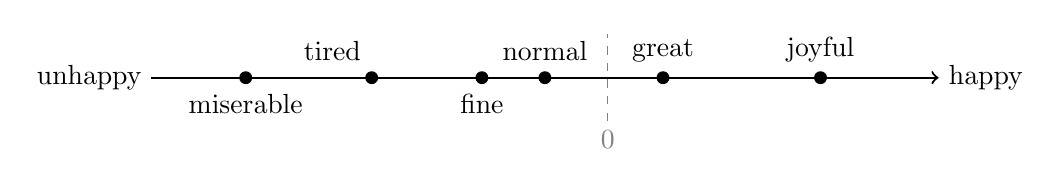
\begin{tikzpicture}
  % Axis: Increased length slightly for better spacing
  \draw[->, thick] (-5,0) -- (5,0) node[right, anchor=west] {happy};
  \node at (-5,0) [left, anchor=east] {unhappy};

  % Origin mark: Made slightly more prominent
  \draw[dashed, gray] (0.8,-0.55) -- (0.8,0.55);
  \node at (0.8,-0.55) [below, gray] {0}; % Added 'below' for clarity

  % Words: Adjusted positions and label placement for clarity
  % Using nodes for points allows easier label anchoring
  \node (miserable) [draw, circle, inner sep=1.5pt, fill=black, label=below:miserable] at (-3.8,0) {}; % Increased distance
  \node (tired)    [draw, circle, inner sep=1.5pt, fill=black, label={[below,yshift=.5cm,xshift=-.5cm]tired}]    at (-2.2,0) {};
  \node (fine)     [draw, circle, inner sep=1.5pt, fill=black, label=below:fine]     at (-0.8,0) {};
  \node (normal)   [draw, circle, inner sep=1.5pt, fill=black, label={[below,yshift=.5cm]normal}]   at (0,0.0) {};
  \node (great)    [draw, circle, inner sep=1.5pt, fill=black, label=above:great]    at (1.5,0) {}; % Adjusted position
  \node (joyful)   [draw, circle, inner sep=1.5pt, fill=black, label=above:joyful]   at (3.5,0) {}; % Adjusted position
\end{tikzpicture}
\end{center}

The word ``fine'' appears on the negative side of the axis, closer to ``unhappy'' than to ``happy.''
The word ``normal'' is semantically neutral and equidistant from ``happy'' and ``unhappy.''
Why is the origin (0) of the embedding space not a reliable indicator of semantic neutrality, even if the pole words (``happy'' and ``unhappy'') were chosen carefully, and the neutral word (e.g., ``normal'') appears at the middle point of the pole words? Provide an example to illustrate your answer (e.g., draw a 2D scatter plot of word embeddings, semantic axis, and the origin).

Grading Criteria (5 points):
\begin{itemize}
  \item (2 points) Identifies why the origin is not a reliable indicator of semantic neutrality.
  \item (3 points) Provide an example to illustrate the answer.
\end{itemize}

\begin{solution}
The origin of the embedding space is arbitrary. Embedding algorithms optimize contextual co-occurrence and do not center semantic meaning around zero. The semantic axis constructed from "unhappy" to "happy" uses these specific words to define a direction, but the geometric origin need not align with semantic neutrality.
\end{solution}

\question[5] Altinok GeBNLP 2024 studies gender bias in word embeddings trained on Turkish, a language that lacks grammatical gender (e.g., it uses a single pronoun for both ``he'' and ``she''). Yet, the study finds significant gender associations in the resulting embeddings. Explain how gender bias can emerge in word embeddings for a gender-neutral language. Your answer should reference at least one mechanism by which such bias is learned during training, and why this challenges the assumption that grammatical neutrality implies embedding neutrality in terms of stereotypes. You may refer to the following examples from the study:
\begin{itemize}
    \item The word ``nurse'' is more closely associated with female names, while ``professor'' is more associated with male names.
    \item The word ``makeup'' is grammatically neutral but clusters with culturally feminine terms in the embedding space.
\end{itemize}

Grading Criteria (5 points):
\begin{itemize}
  \item (2 points) Clearly explains a process by which gender bias is learned during training.
  \item (3 points) Explains why grammatical neutrality does not guarantee embedding neutrality.
\end{itemize}

\begin{solution}
This happens because embeddings learn from patterns in how words appear together in large amounts of text. If certain words frequently appear in contexts that reflect real-world gender roles or stereotypes, the embeddings will capture those associations.
For example, if the word ``nurse'' often appears near female names, and ``professor'' near male names, embeddings will reflect that pattern by associating each word with a specific gender. Similarly, a word like ``makeup,'' which is grammatically neutral, may still appear in contexts involving femininity and therefore be embedded closer to female-associated terms.
Thus, grammatical neutrality doesn't prevent bias—models pick up on how language is used in society.
\end{solution}

\question[5] In Transformer architectures, layer normalization plays a critical role in stabilizing training. The layer normalization is defined by:

\begin{align*}
  \hat{x}_i &= \gamma \frac{x_i-\mu_i}{\sqrt{\sigma_i^2+\epsilon}} + \beta_i,
\end{align*}
where \(\mu_i\) is the mean and \(\sigma_i\) is the standard deviation of the input \(x_i\), \(\epsilon\) is a small constant to prevent division by zero, and \(\gamma\) and \(\beta\) are learnable parameters.
Apply the layer normalization with $(\epsilon, \gamma, \beta) = (0, 1, 1)$ to the following data points and draw the normalized data points as 2D scatter plot. Show your work.

Grading Criteria (5 points):
\begin{itemize}
  \item (3 points) Correctly applies the layer normalization formula.
  \item (2 points) Correctly plots the normalized data points.
\end{itemize}

\begin{center}
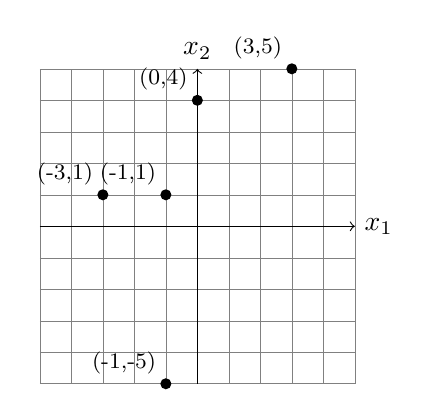
\begin{tikzpicture}[scale=0.4]
  % Draw grid with 1 cm spacing
  \draw[step=1cm,gray,very thin] (-5,-5) grid (5,5);
  % Draw the x and y axes
  \draw[->] (-5,0) -- (5,0) node[right] {$x_1$};
  \draw[->] (0,-5) -- (0,5) node[above] {$x_2$};
  % Plot and label the data points
  \foreach \x/\y in {-1/-5, 3/5, -1/1, -3/1, 0/4} {
    \fill (\x,\y) circle (5pt);
    \node[above left, font=\footnotesize] at (\x,\y) {(\x,\y)};
  }
\end{tikzpicture}
\end{center}

\begin{solution}

\begin{center}
    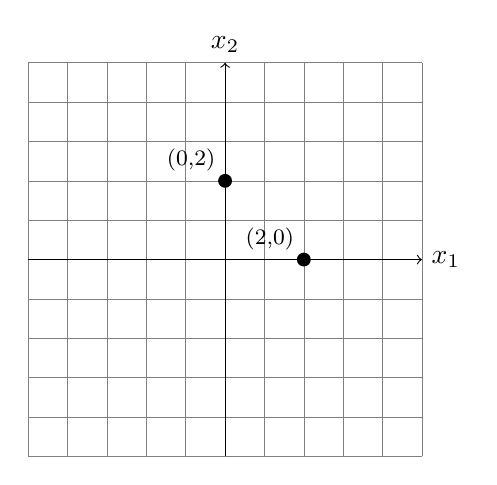
\begin{tikzpicture}[scale=0.5]
      % Draw grid with 1 cm spacing
      \draw[step=1cm,gray,very thin] (-5,-5) grid (5,5);
      % Draw the x and y axes
      \draw[->] (-5,0) -- (5,0) node[right] {$x_1$};
      \draw[->] (0,-5) -- (0,5) node[above] {$x_2$};
      % Plot and label the data points
      \foreach \x/\y in {0/2, 2/0} {
        \fill (\x,\y) circle (5pt);
        \node[above left, font=\footnotesize] at (\x,\y) {(\x,\y)};
      }
    \end{tikzpicture}
\end{center}

\end{solution}


%\question[4] Consider a BERT-based model handling text inputs. Answer the following:
%
%\begin{enumerate}
%  \item (1 points) Where does the [CLS] token go in a given text?
%  \item (1 points) Where does the [SEP] token go in a given text?
%  \item (1 points) Explain the purpose of the [MASK] token in the masked language modeling task.
%  \item (1 points) Provide a specific example of a sentence that includes the [CLS], [SEP], and [MASK] tokens. Explain the function of each token in your example.
%\end{enumerate}
%
%\begin{solution}
%\begin{enumerate}
%  \item \textbf{[CLS] Token (1 points):}
%    The [CLS] token is added at the beginning of an input sequence. It aggregates contextual information from the entire sequence and serves as the basis for classification tasks.
%
%  \item \textbf{[SEP] Token (1 points):}
%    The [SEP] token marks the boundary between segments, enabling BERT to distinguish among separate sentences or parts of the input. It is essential for tasks involving sentence pairs.
%
%  \item \textbf{[MASK] Token (1 points):}
%    During the masked language modeling pre-training, the [MASK] token replaces selected words. BERT is trained to predict these masked tokens by leveraging the surrounding context, leading to robust bidirectional representations.
%
%  \item \textbf{Example (1 points):}
%    Consider the sentence:
%    ``[CLS] The chef prepared a [MASK] meal. [SEP] The meal was awesome.''
%    Here, the [CLS] token signals the start of the input and aggregates contextual features for classification; the [MASK] token replaces an expected descriptor (e.g., "delicious"), which the model must predict during pre-training; the [SEP] token indicates the end of the segment, ensuring clear segmentation.
%\end{enumerate}
%\end{solution}


\question[8] Imagine you're tasked with creating an instruction-based prompt to help an LLM deliver an insightful movie review for a specific film. The intended audience is general moviegoers seeking a balanced analysis of the film's strengths and weaknesses. Construct a prompt that incorporates the following key components: Instruction, Data, Output Indicator, Persona, Context, and Audience. In your answer, \ul{outline how each component contributes to a clear and effective review}. For the prompt, explicitly specify the context, persona, output indicator, and audience.

Grading Criteria (8 points):
\begin{enumerate}
  \item (1 point for each component) Explain how each component impacts the LLM's output.
  \item (2 points) Create a complete prompt that explicitly includes all six components.
\end{enumerate}


\begin{solution}
\begin{itemize}
   \item \textbf{Instruction} defines what the LLM should do.
   \item \textbf{Data} provides essential background information needed to complete the task effectively.
   \item \textbf{Output Indicator} specifies the expected format and structure of the response.
   \item \textbf{Persona} establishes the tone, perspective, and voice the LLM should adopt.
   \item \textbf{Context} sets the situational background and relevant circumstances for the task.
   \item \textbf{Audience} identifies who will be reading the output, helping tailor the content appropriately.
\end{itemize}

\textbf{Prompt:}

\begin{quote}
\textbf{Persona:} You are a movie critic who is known for your clear, balanced, and engaging commentary.
\textbf{Instruction:} Write a detailed movie review for the film The Midnight Escape.
\textbf{Data:} Include information from the provided synopsis, key scenes, and highlighted themes.
\textbf{Output Indicator:} The review must end with an overall rating out of 10 and a bulleted list summarizing the film’s major strengths and weaknesses.
\textbf{Context:} This review is intended for a modern audience that appreciates thoughtful analysis of both narrative and technical aspects without requiring specialized knowledge.
\textbf{Audience:} General moviegoers who seek comprehensive yet accessible film critiques.
\end{quote}
\end{solution}
\end{questions}

\end{document}
